\documentclass[11pt]{article}
\usepackage[margin=0.78in]{geometry}
\usepackage{amsmath,amssymb,booktabs,graphicx,microtype,xcolor}
\usepackage[hidelinks]{hyperref}
\usepackage[font=small,labelfont=bf]{caption}
\usepackage{enumitem}
\definecolor{atlasblue}{HTML}{176B87}
\hypersetup{colorlinks=true,linkcolor=atlasblue,citecolor=atlasblue,urlcolor=atlasblue}
\setlength{\parindent}{0pt}
\setlength{\parskip}{5pt}
\setlist[itemize]{leftmargin=1.3em,itemsep=2pt,topsep=3pt}
\newcommand{\fedd}{f_{\mathrm{Edd}}}
\newcommand{\mbh}{M_{\mathrm{BH}}}
\newcommand{\mseed}{M_{\mathrm{seed}}}

\title{\textbf{The High-Redshift Accretion Atlas}\\
\large Reproducible Catalogue and Class-Aware Growth Diagnostics, Release v7.5}
\author{Nicole Jiang}
\date{27 August 2026}

\begin{document}
\maketitle

\begin{abstract}
We present v7.5 of a provenance-aware atlas of reported accreting black holes at
$z\geq4$. The release contains 234 literature measurements representing 219
physical objects in 218 host systems. Its science layer uses 209 measurements
and 196 preferred physical-object rows with canonical numeric black-hole masses;
23 catalogue objects without such masses remain explicit exclusions. The atlas
keeps heterogeneous evidence classes and mass methods separate, retains
alternate measurements, and treats global ranks as navigation rather than
demographic inference. A full-source audit corrects the Scholtz et al. JADES
narrow/high-ionization subset to 21 objects at $z\geq4$ and documents the
paper/table count discrepancy without altering frozen v7.4 artifacts. Under the
reference assumptions $z_{\rm seed}=30$, $\epsilon=0.1$, and no merger boost,
luminous quasars occupy the highest growth-pressure region. These diagnostics
measure pressure under stated assumptions; they do not identify a unique seed or
accretion history.
\end{abstract}

\section{Purpose and interpretation boundary}

The atlas asks which reported objects place the strongest pressure on simple
black-hole growth histories, and which measurements most affect that conclusion.
It does not estimate a population mass function from the pooled catalogue. The
input literature spans broad-line AGN selected by several JWST surveys
\cite{juodzbalis2026,taylor2025,matthee2024,lin2024,harikane2023,davis2026},
luminous-quasar comparison samples \cite{mazzucchelli2023,shen2019}, host-selected
broad-line candidates \cite{ren2025}, an X-ray evidence history
\cite{bogdan2024,zou2026}, and JADES narrow/high-ionization candidates
\cite{scholtz2025}. Selection functions, evidence strength, and mass estimators
are therefore retained as analysis strata.

\section{Catalogue construction and provenance}

Every measurement has a stable measurement ID, physical-object ID, and host
system ID. Source-native values, adopted canonical values, uncertainty kinds,
method tags, URLs, available archive checksums, and identity decisions are
preserved. Missing historical provenance is explicit: the 23 frozen-v1
Juod\v{z}balis/JADES rows predate archive hashing and retain a documented
unavailable checksum and extraction-date limitation rather than a fabricated
value. Auxiliary coordinate and context inputs are attributed separately to the
E-XQR-30 survey catalogue \cite{dodorico2023}, the THRILS programme catalogue
\cite{hutchison2025}, the UHZ1 spectroscopy paper \cite{goulding2023}, and the
versioned JADES DR3 GOODS-S prism catalogue.
Alternate measurements are never silently averaged or deleted. Exactly one
preferred measurement controls each object-level status in v7.5, while the
complete history of measurement-level evidence statuses and bases remains in the
object table. This resolves the case in which a weaker alternate candidate row
had conservatively downgraded an otherwise secure preferred measurement.

The Scholtz et al. source audit deserves specific note. The paper reports 42
objects, while its source-native sample table contains 41 rows. Parsing that full
table gives exactly 21 rows at $z\geq4$. Frozen v7.4 contained 20 of them; v7.5
adds the omitted JADES-NS-GS00099671 row ($z=5.936$) with its published host and
bolometric observables, but no invented black-hole mass. The 21 candidates
include one identity-linked broad-line object, so the current physical-object
catalogue contains 20 narrow-line candidates from this source.

\begin{table}[ht]
\centering
\caption{Current v7.5 release scale and explicit analysis subsets.}
\begin{tabular}{@{}lr@{}}
\toprule
Product or subset & Rows / objects \\
\midrule
Measurements / physical objects / host systems & 234 / 219 / 218 \\
Source-local observables & 1,106 \\
Growth-eligible measurements / objects & 209 / 196 \\
Primary measurements / objects & 182 / 171 \\
Broad-line / luminous-quasar eligible objects & 112 / 84 \\
Catalogue-only physical objects & 23 \\
Alternate-measurement sensitivity pairs & 13 \\
Per-object growth images / compiled class grids & 588 / 6 \\
\bottomrule
\end{tabular}
\end{table}

\begin{figure}[p]
\centering
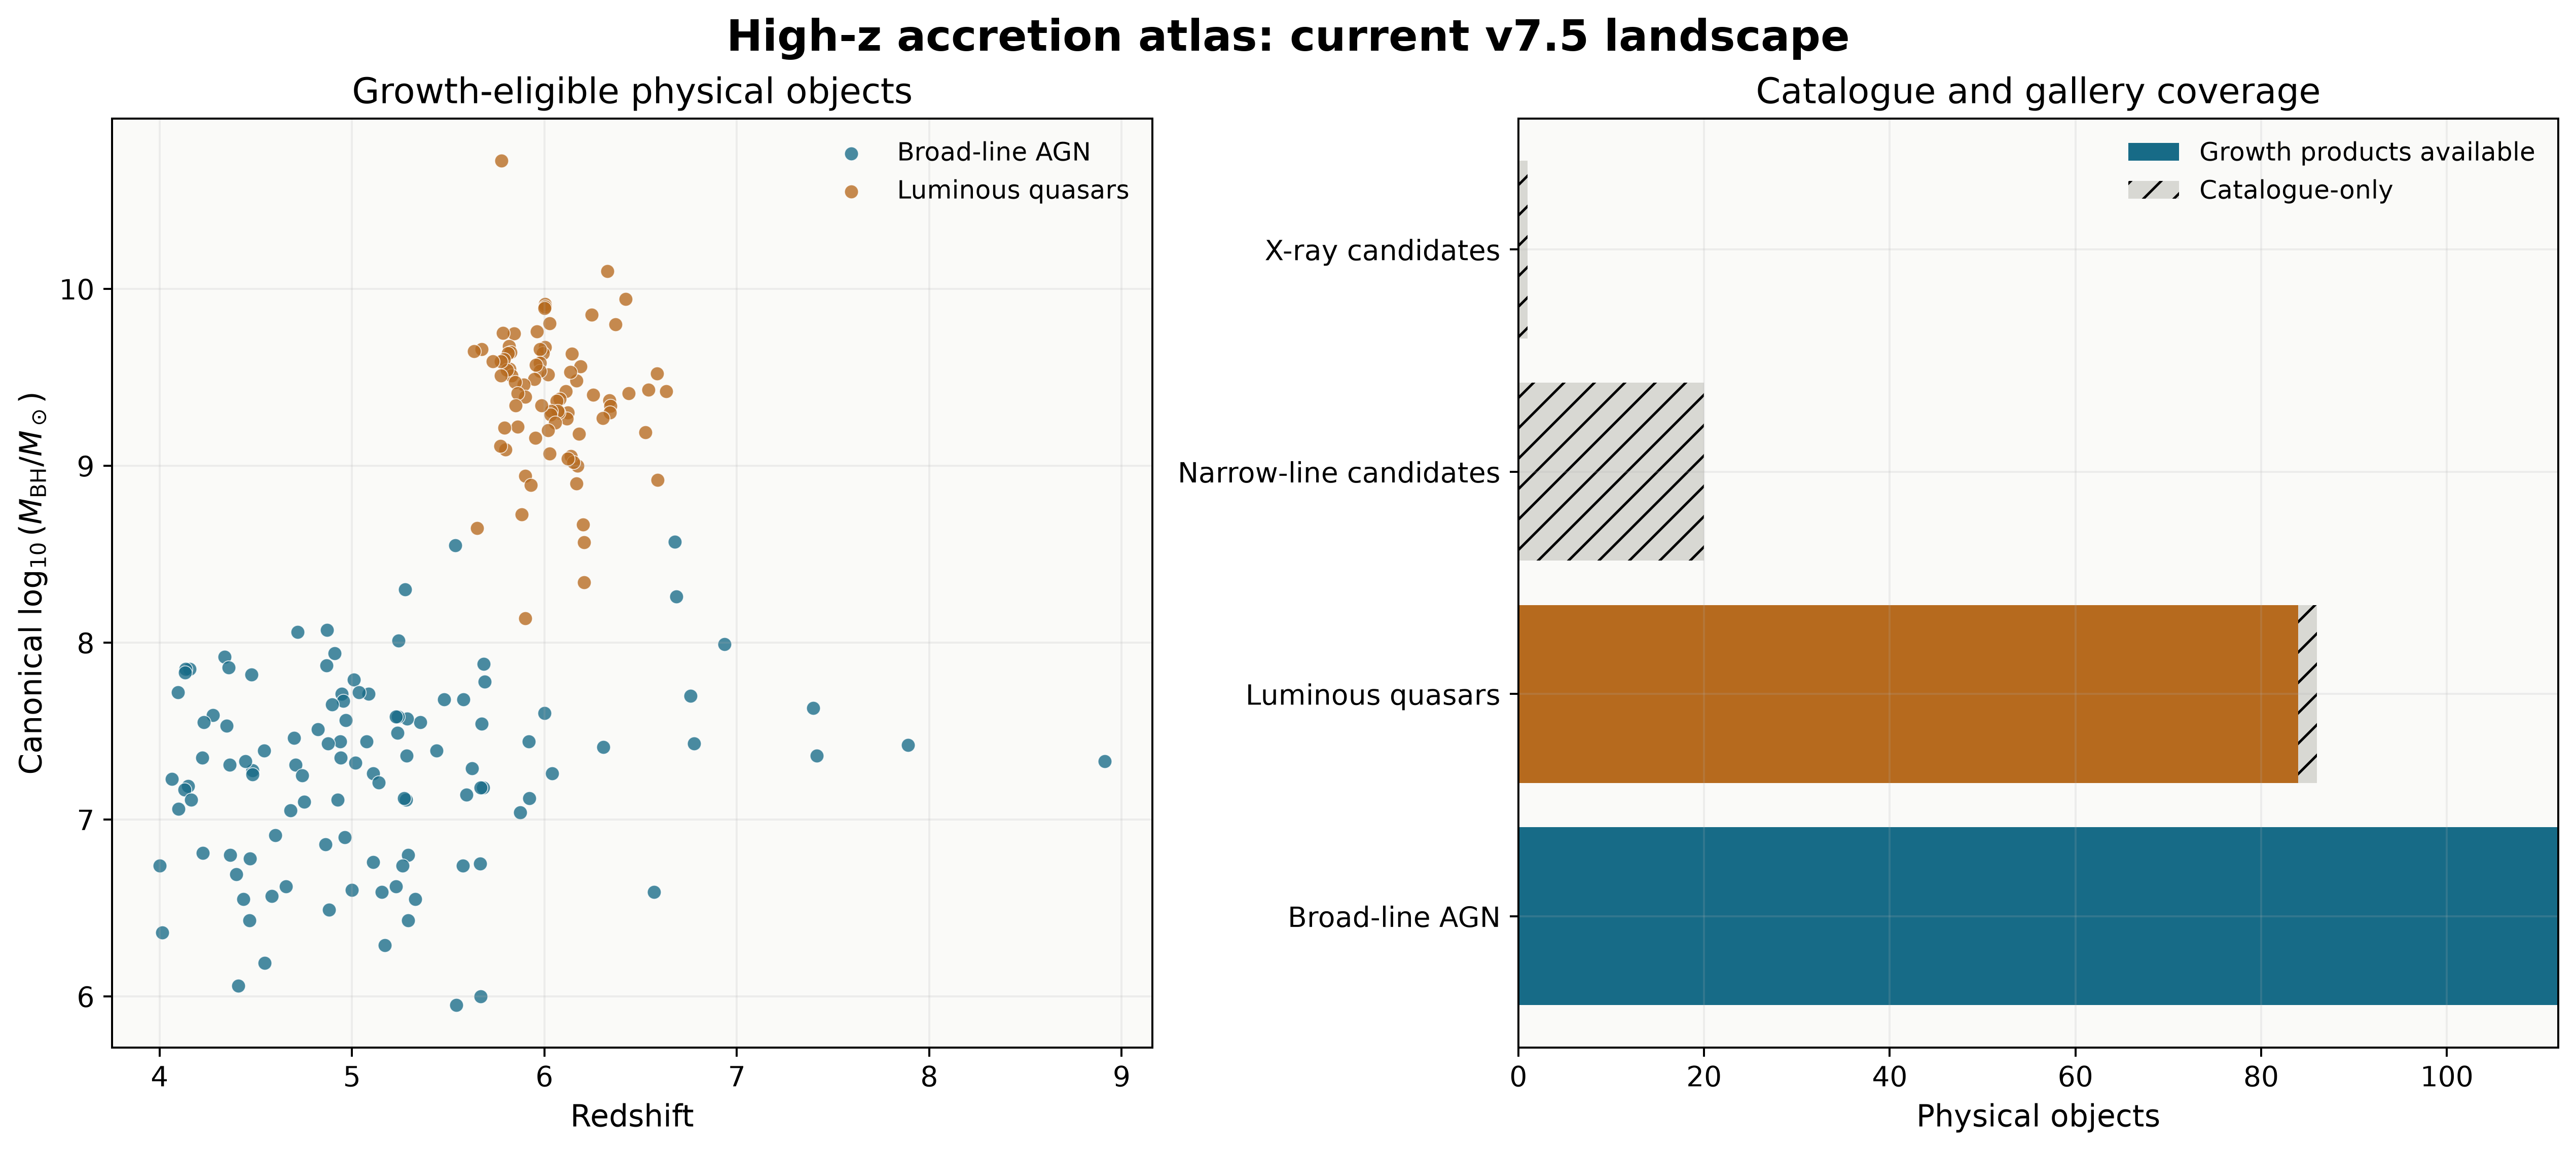
\includegraphics[width=0.99\textwidth]{../results/figures/v7_5_catalogue_growth_landscape.png}
\caption{Current catalogue landscape. Left: all 196 growth-eligible physical
objects in black-hole-mass--redshift space. Right: growth-product coverage for
all 219 objects. The 23 catalogue-only objects remain available for provenance
and evidence analyses but are not assigned numeric growth products.}
\label{fig:landscape}
\end{figure}

\section{Growth model and uncertainty}

The reference model follows exponential radiatively efficient growth
\cite{dayal2024},
\begin{equation}
\mbh(t_{\rm obs})=\mseed\exp\left[\fedd
\left(\frac{1-\epsilon}{\epsilon}\right)
\frac{t(z_{\rm obs})-t(z_{\rm seed})}{t_{\rm Edd}}\right]B_{\rm merge},
\end{equation}
with $t_{\rm Edd}\simeq0.45$ Gyr. The main tables invert this relation to report
required lifetime-average $\fedd$ for fixed seed masses and required $\mseed$ for
fixed $\fedd$. The baseline uses $z_{\rm seed}=30$, $\epsilon=0.1$, and
$B_{\rm merge}=1$.

Reported asymmetric statistical uncertainties in $\log_{10}\mbh$ are propagated
with 10,000 deterministic, per-object split-side draws. Method-scale systematic
envelopes remain separate from the statistical sampling. A reported current
Eddington ratio is not substituted for the lifetime-average growth rate.

\begin{figure}[p]
\centering
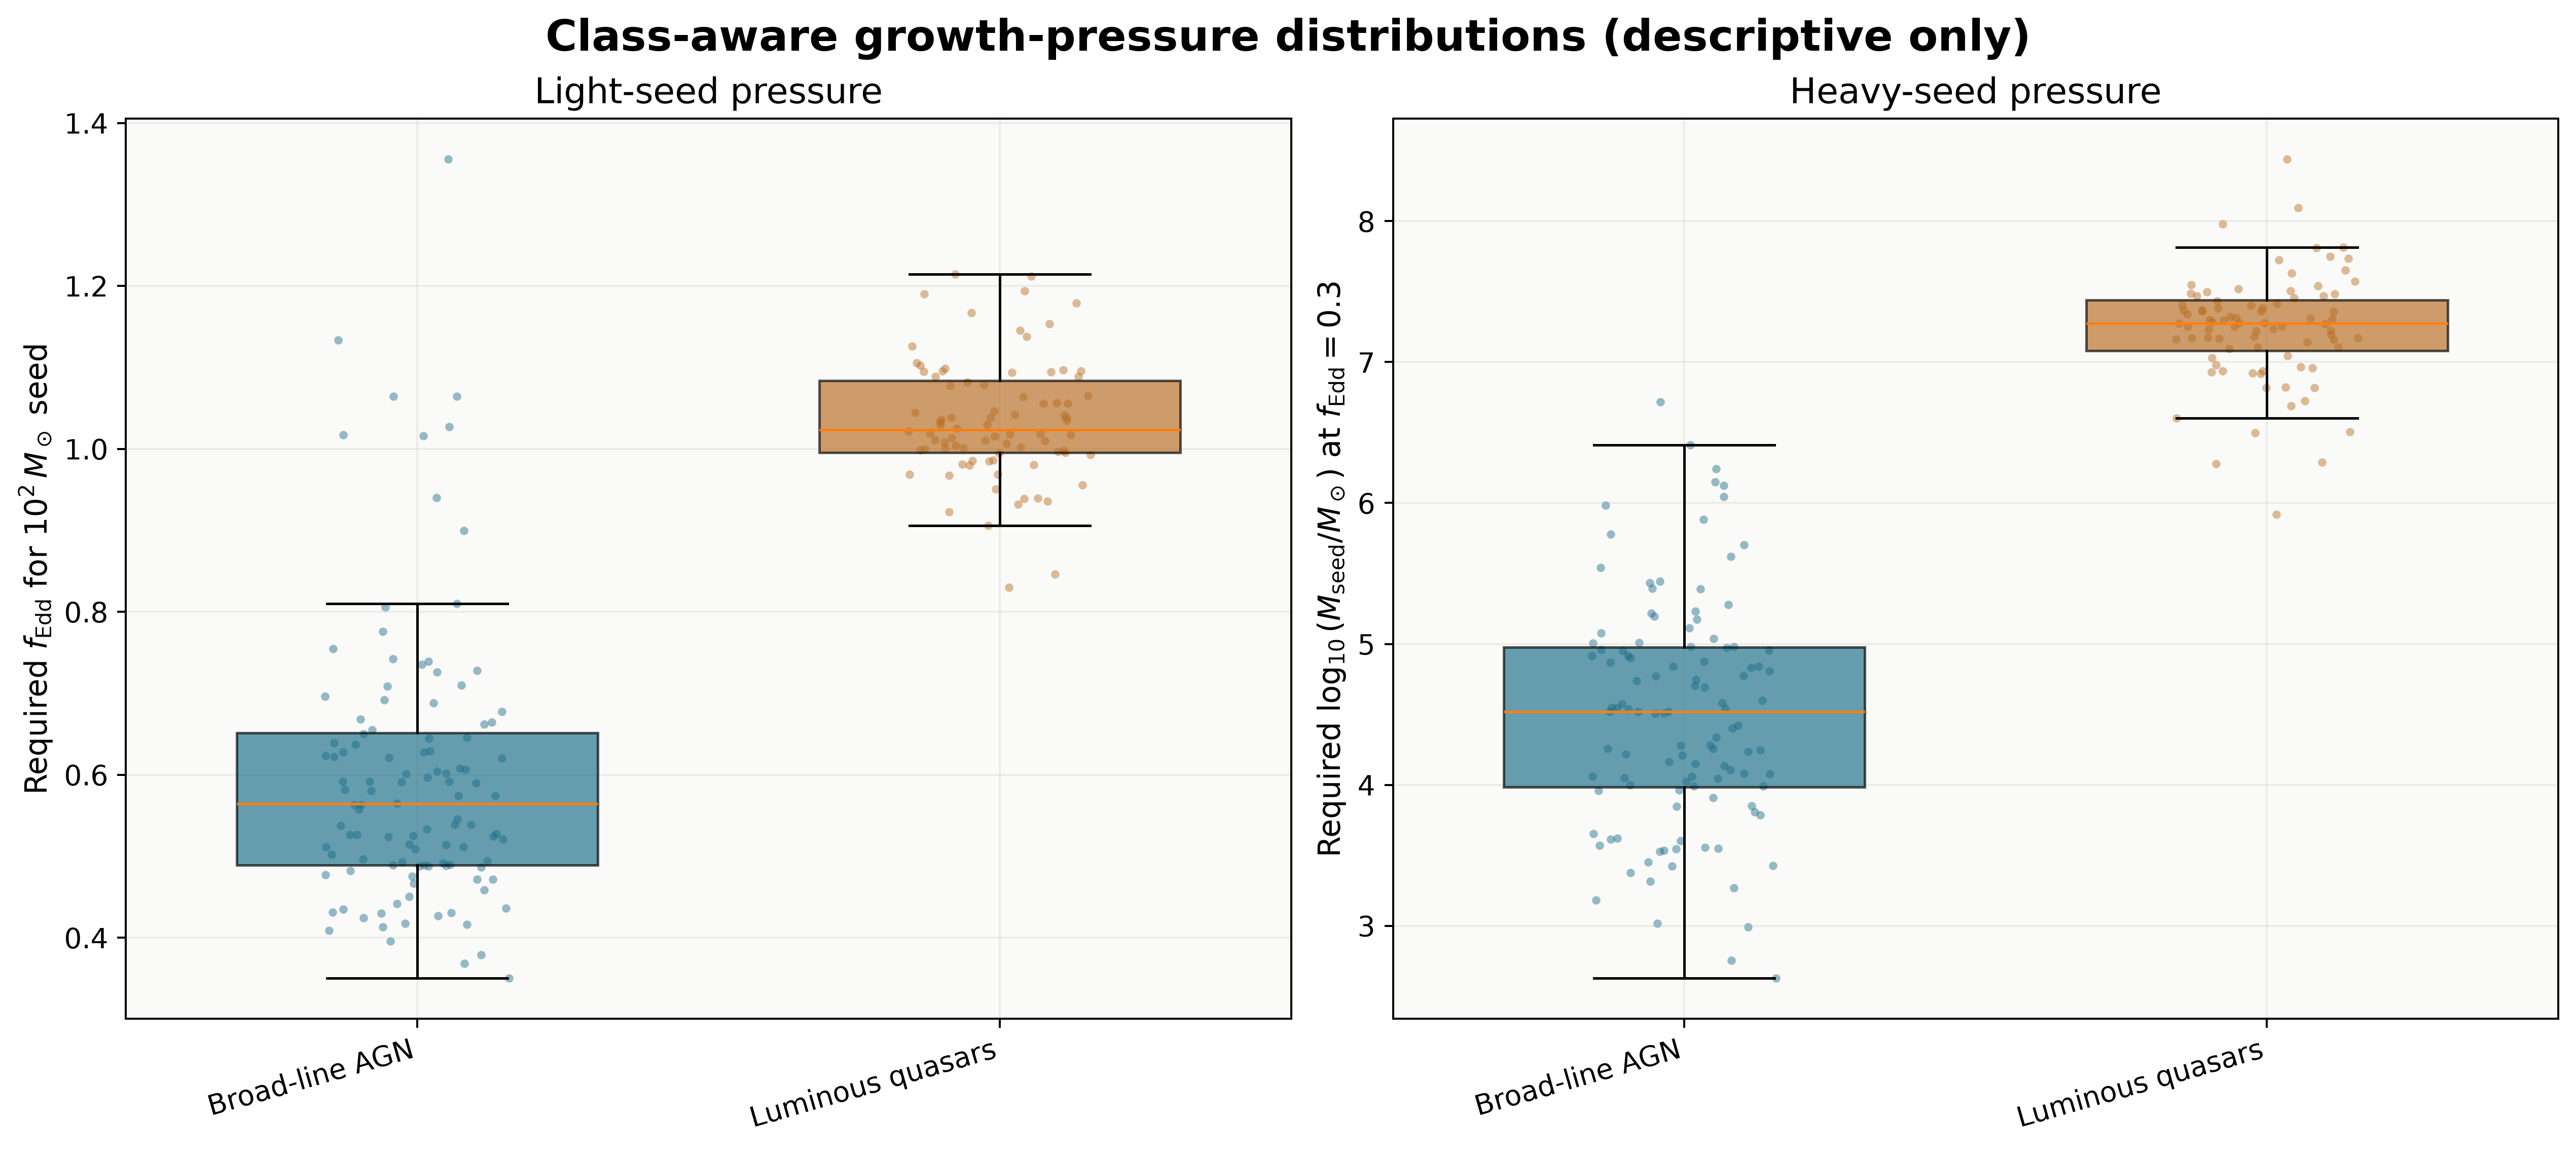
\includegraphics[width=0.99\textwidth]{../results/figures/v7_5_class_aware_growth_pressure.png}
\caption{Descriptive class-aware growth-pressure distributions. The luminous
quasar comparison sample and faint broad-line AGN are shown separately because
their selection functions and mass regimes differ. Boxes and points summarize
the released object-level table; they are not completeness-corrected demographic
estimates.}
\label{fig:classes}
\end{figure}

\section{Current results}

The global navigation view places luminous quasars at the highest reference
growth pressure. J1148+5251 is first in the point and uncertainty-aware views,
with median required $\fedd=1.214$ for a $10^2\,M_\odot$ seed. SDSS J0100+2802
and PSO J231-20 follow. The top eight uncertainty-ranked objects have unit
Monte Carlo probability, to the stored precision, of requiring $\fedd>1$ under
the same light-seed reference. These results express tension with that reference
history, not a claim of literally continuous super-Eddington accretion.

Within-class and within-class--mass-method ranks are the supported comparison
scopes. All outputs explicitly forbid pooled demographic inference without a
selection-function and completeness model. The alternate-measurement table
contains 13 comparisons; it shows how retained measurement choice changes
$\log_{10}\mbh$ and required $\fedd$ while leaving the default-release choice
auditable.

\begin{figure}[p]
\centering
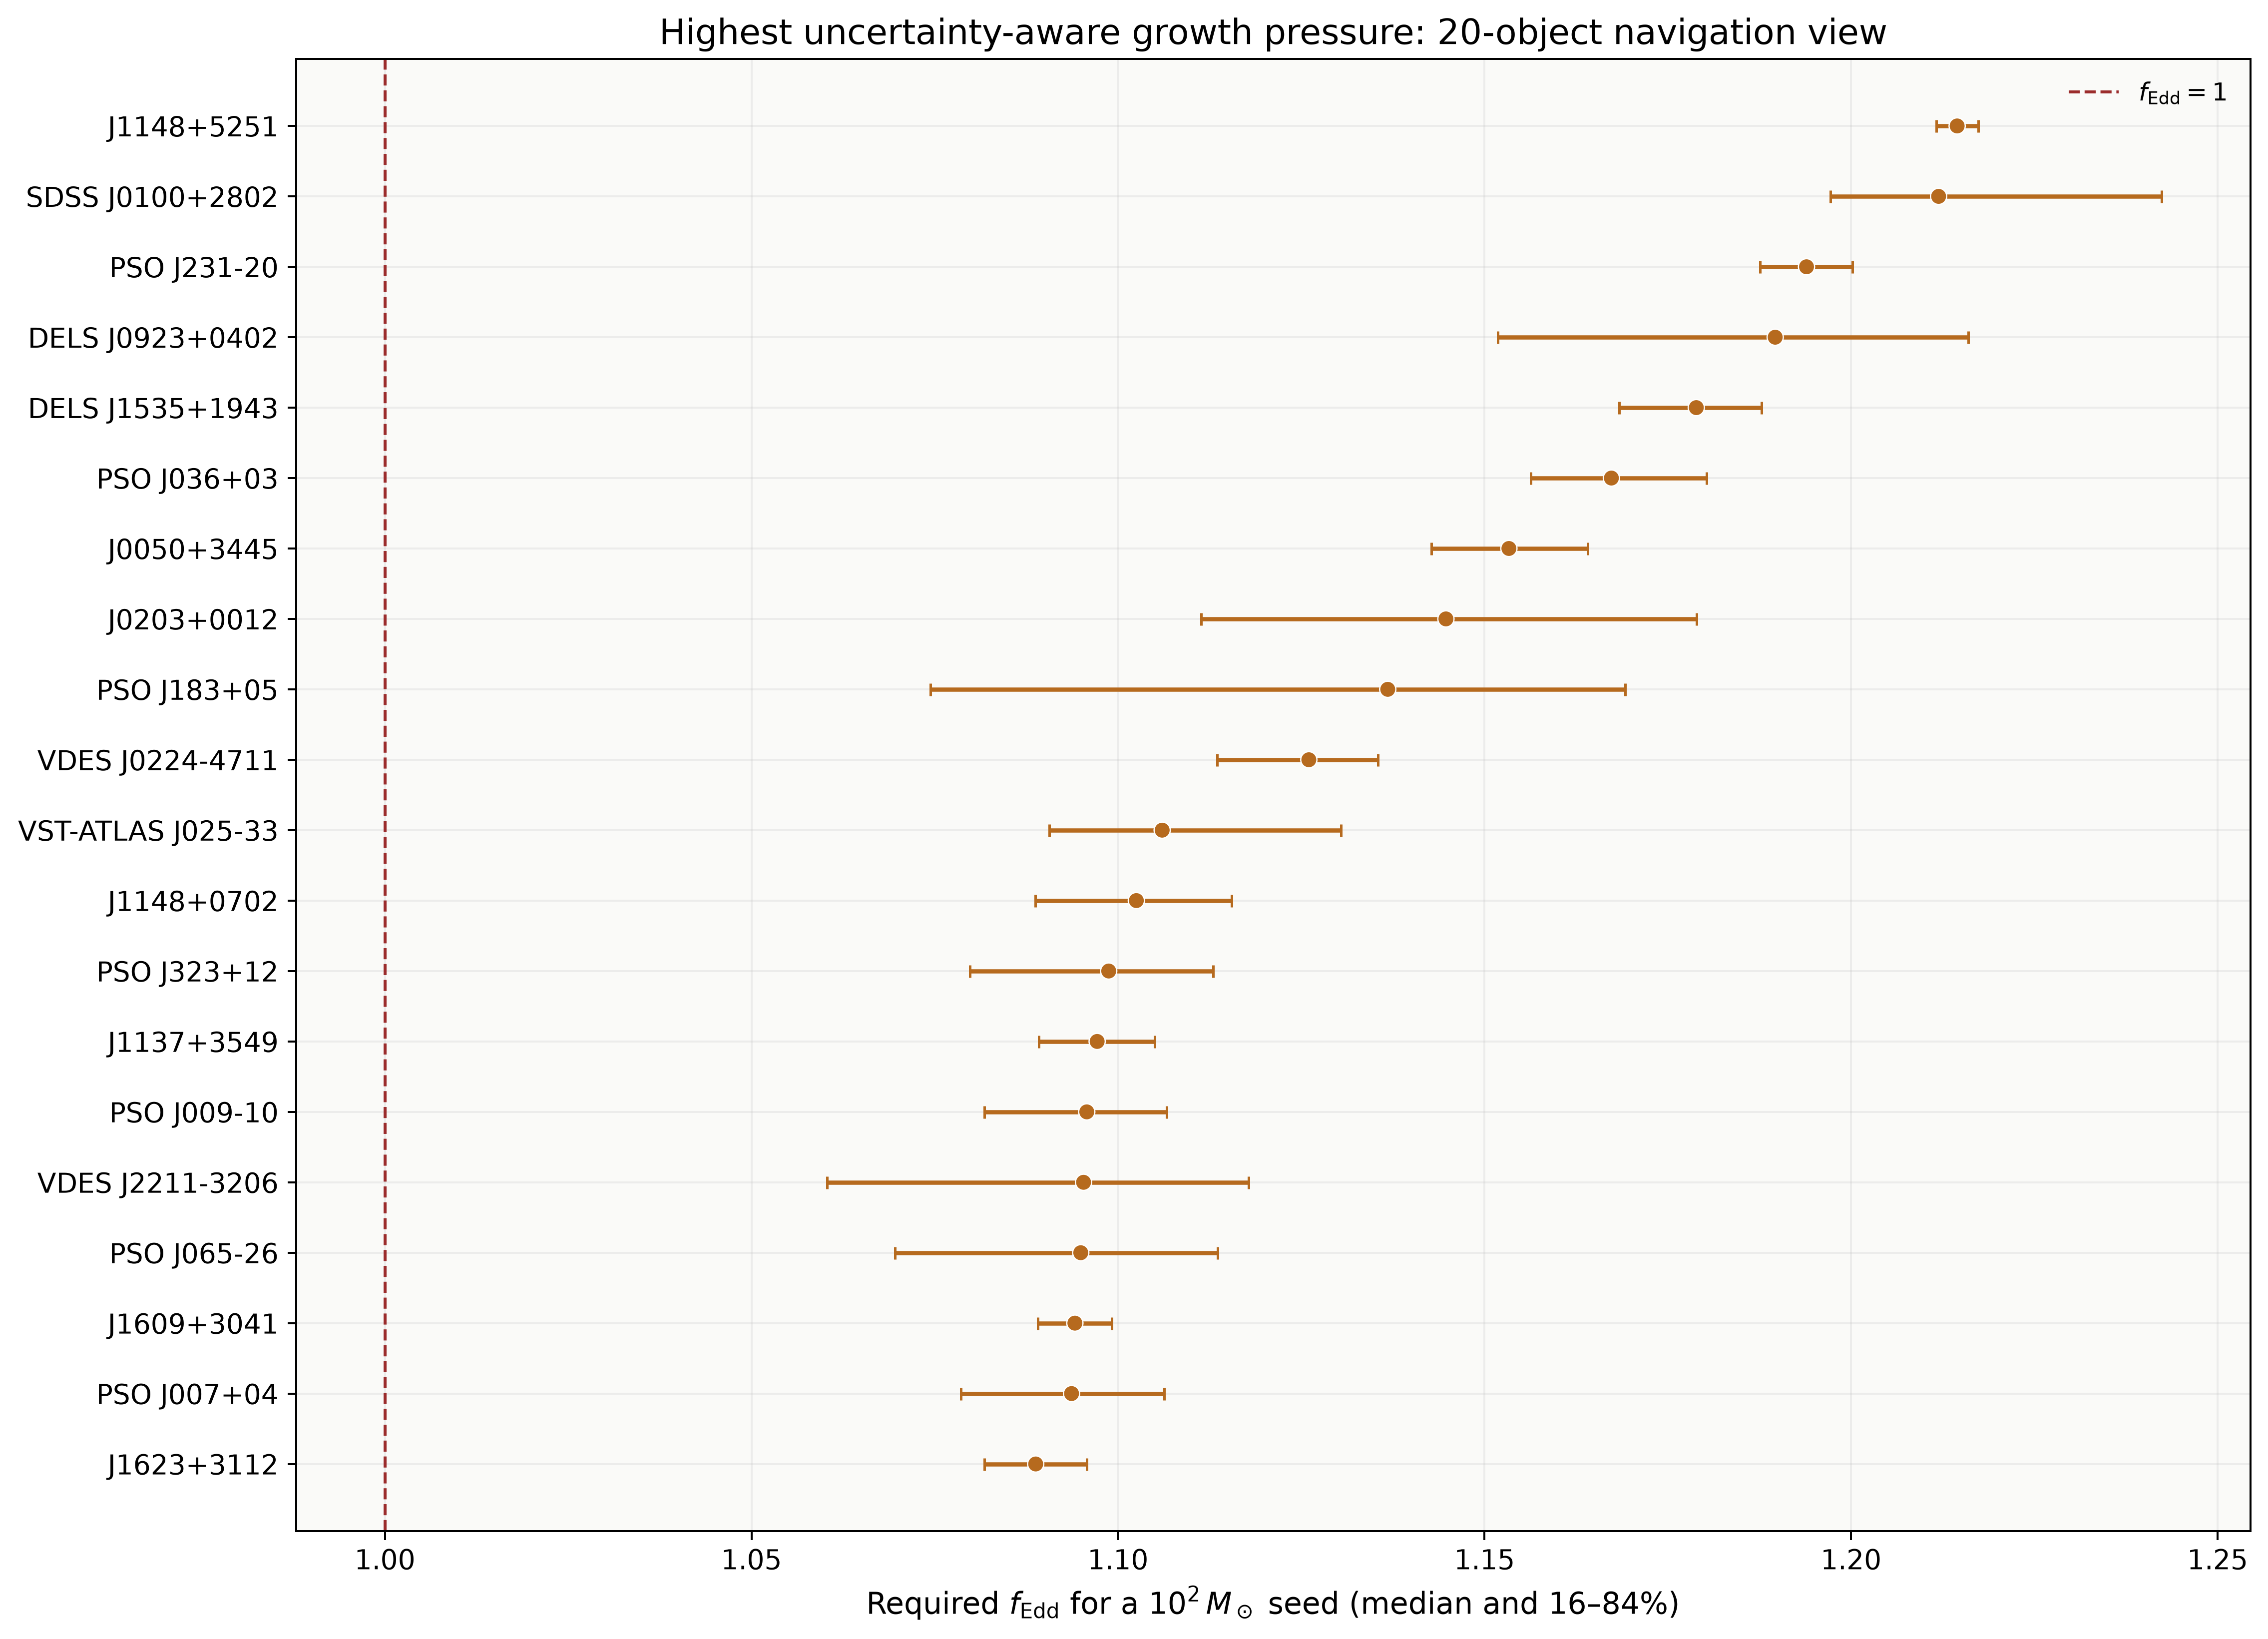
\includegraphics[width=0.97\textwidth]{../results/figures/v7_5_uncertainty_robustness.png}
\caption{Twenty highest uncertainty-aware navigation entries. Points and bars
show the median and 16th--84th percentiles of required $\fedd$ for a
$10^2\,M_\odot$ seed. The dashed line marks $\fedd=1$. Ranking is descriptive
within the released assumptions.}
\label{fig:uncertainty}
\end{figure}

\begin{figure}[p]
\centering
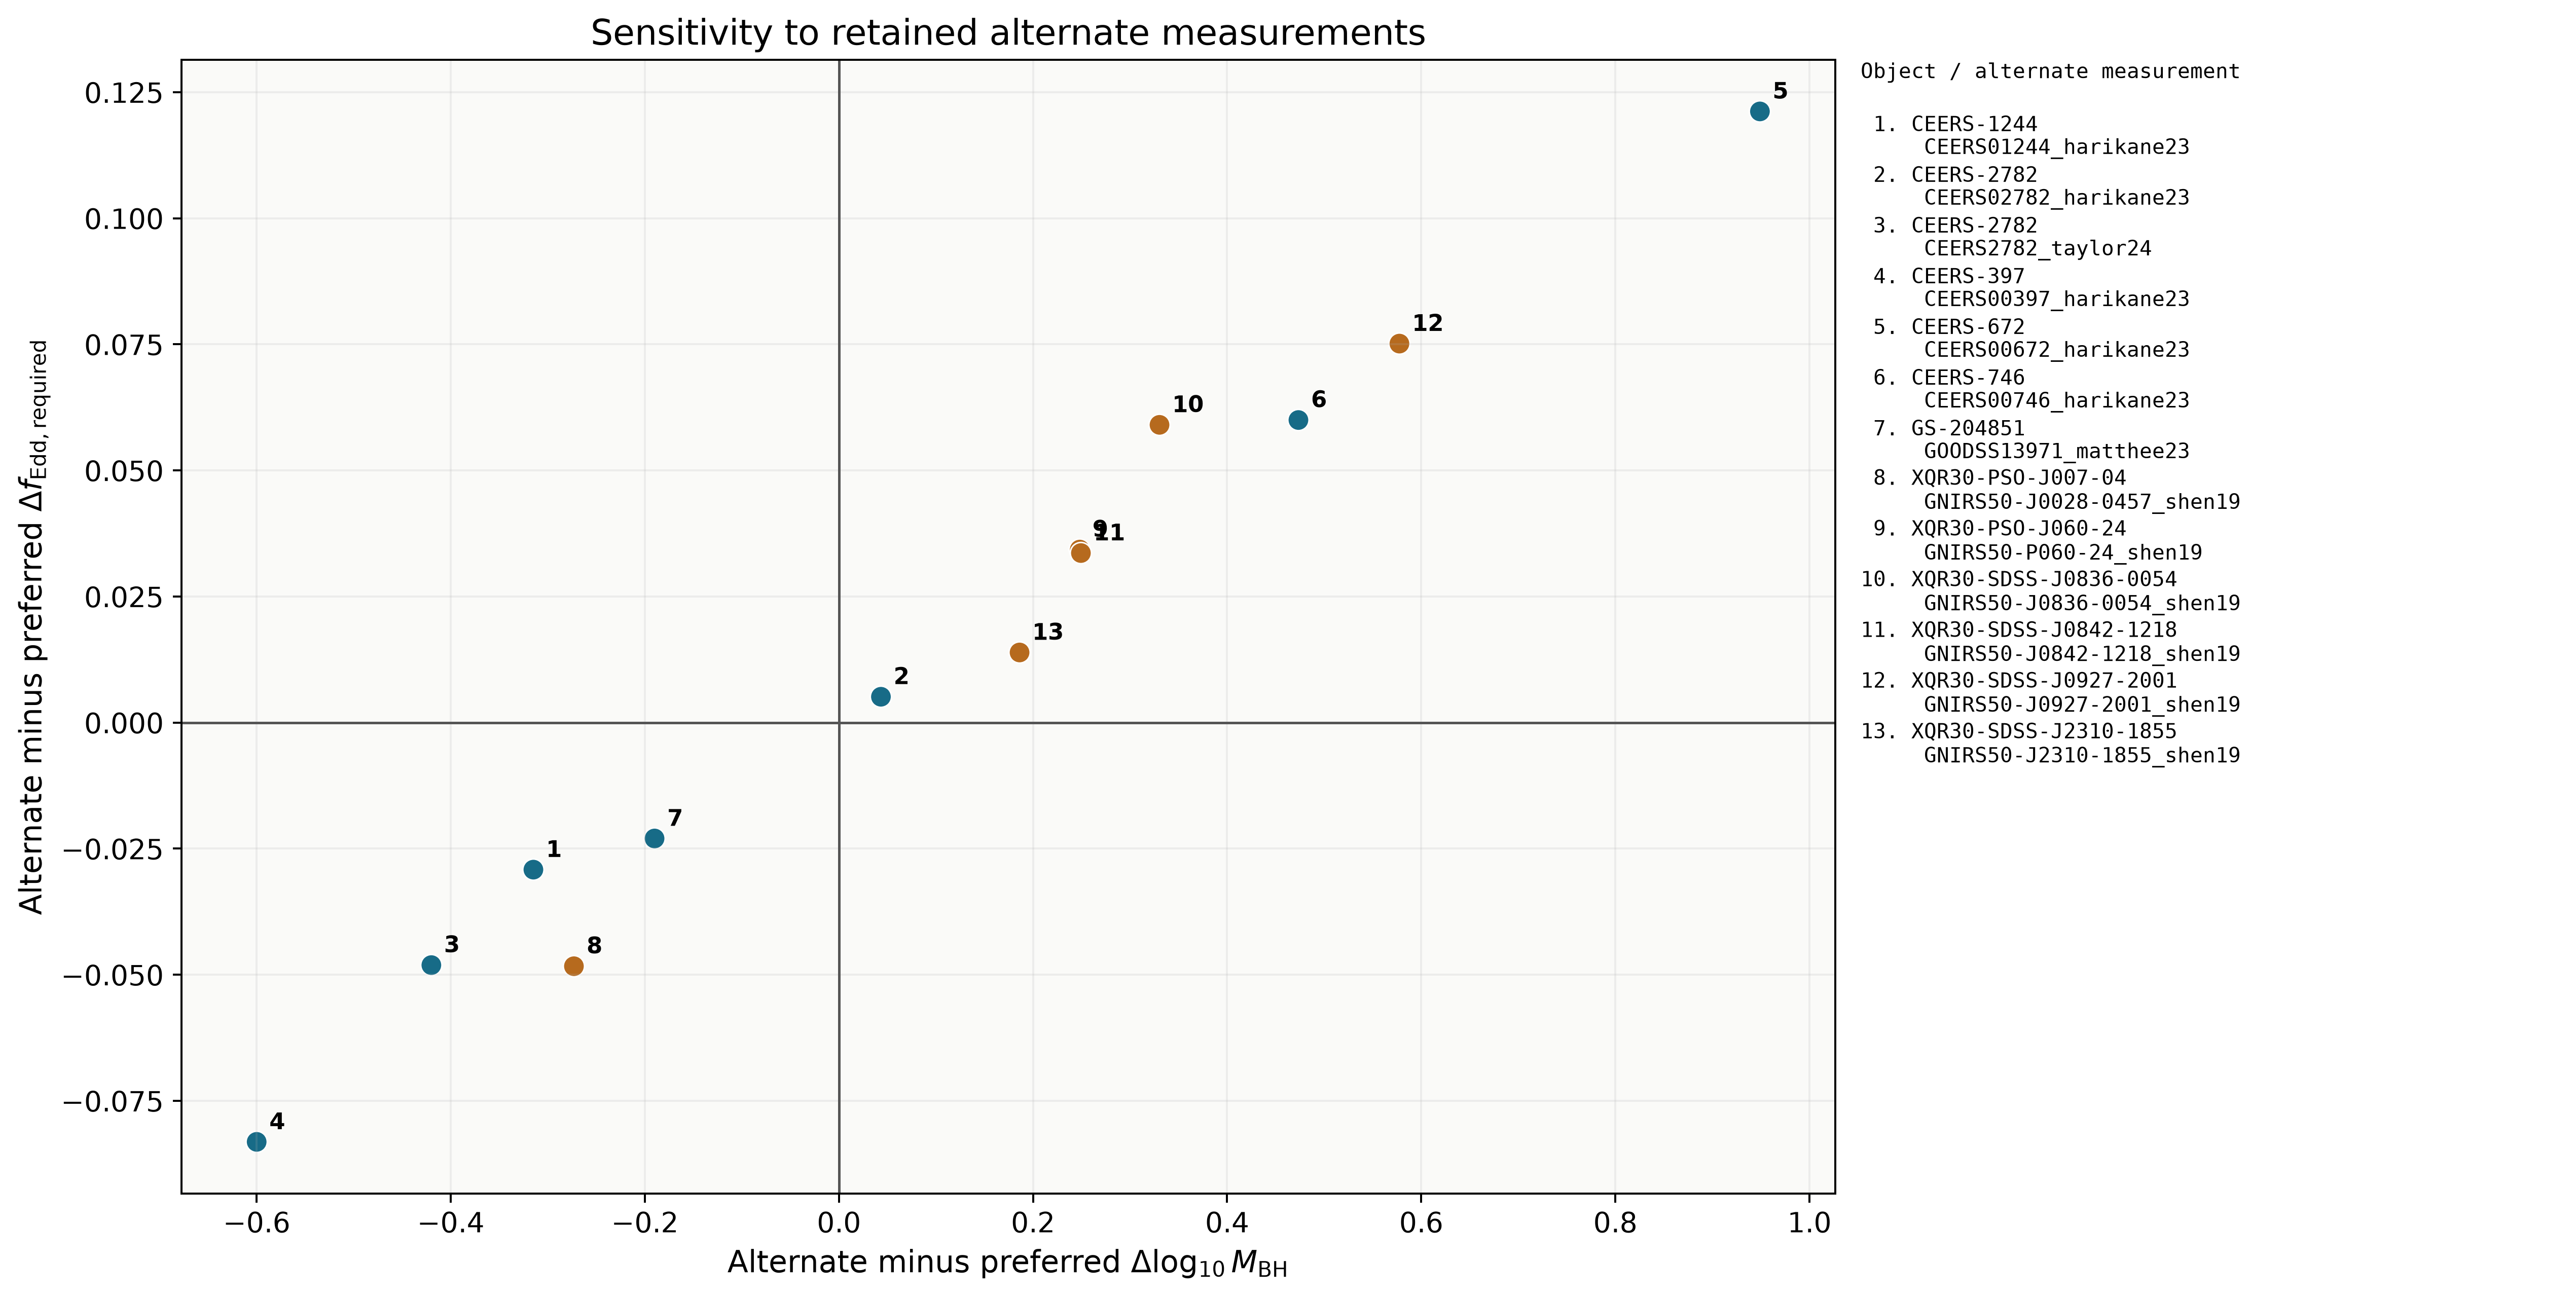
\includegraphics[width=0.99\textwidth]{../results/figures/v7_5_measurement_sensitivity.png}
\caption{Sensitivity to 13 retained alternate measurements. Numbered points are
keyed to stable object and measurement IDs, avoiding ambiguous overlapping
labels. The plot quantifies release-choice sensitivity rather than treating
alternates as independent objects.}
\label{fig:sensitivity}
\end{figure}
\clearpage

\section{Reproducibility and released artifacts}

The Python 3.12 environment is exactly pinned. Catalogue, science, and figure
manifests verify exact artifact membership and SHA-256 hashes. In-memory
reproduction compares generated tables against checked-in CSVs without rewriting
them. Regression tests enforce cardinalities, source anchors, identity links,
evidence aggregation, uncertainty boundaries, ranking policy, figure resolution,
and every inherited gallery path. Frozen releases remain independently
verifiable.

The v7.5 figure layer provides four paper-facing figures. Its coverage table
points to the byte-identical v7.4 per-object gallery because the 196 eligible
objects and their growth inputs are unchanged. That gallery contains a parameter
map, seed-redshift map, and growth track for each eligible object, plus six
high-resolution class grids intended for close zooming. The 23 unavailable
objects are recorded explicitly.

\section{Limitations and next scientific work}

\begin{itemize}
\item The catalogue is heterogeneous and cannot support pooled demographics
without explicit selection and completeness models.
\item Virial masses are method-dependent; available method systematics are
reported separately and are not full posterior reconstructions.
\item Narrow-line and X-ray candidates without canonical numeric masses are
valuable evidence records but cannot enter the current growth ranking.
\item The reference model compresses time-variable accretion, feedback, mergers,
and radiative-state changes into effective parameters.
\item Identity review uses deterministic candidates and documented decisions;
crowded or imprecise cases may ultimately require probabilistic crossmatching.
\end{itemize}

The next scientific milestone is no longer basic catalogue assembly. It is a
selection-aware inference layer: explicit survey selection functions,
completeness modeling, method-calibrated hierarchical uncertainty, and an
observing-priority matrix tied to which measurement would most change each
object's physical interpretation.

\section{Conclusion}

v7.5 is a complete, internally consistent research release: the current
catalogue, class-aware science tables, paper figures, full gallery coverage,
provenance correction, evidence policy, and automated verification all refer to
the same release. It provides reproducible observational triage across 219
objects while keeping unsupported demographic and formation-channel claims
outside the scope of the data product.

\begin{thebibliography}{99}
\bibitem{dayal2024} Dayal, P. 2024, \emph{A\&A}, 690, A182, doi:10.1051/0004-6361/202451481.
\bibitem{juodzbalis2026} Juod\v{z}balis, I. et al. 2026, \emph{MNRAS}, 546, stag086, doi:10.1093/mnras/stag086.
\bibitem{taylor2025} Taylor, A. J. et al. 2025, \emph{ApJ}, 986, 165, doi:10.3847/1538-4357/add15b.
\bibitem{matthee2024} Matthee, J. et al. 2024, \emph{ApJ}, 963, 129, doi:10.3847/1538-4357/ad2345.
\bibitem{lin2024} Lin, X. et al. 2024, \emph{ApJ}, 974, 147, doi:10.3847/1538-4357/ad6565.
\bibitem{harikane2023} Harikane, Y. et al. 2023, \emph{ApJ}, 959, 39, doi:10.3847/1538-4357/ad029e.
\bibitem{davis2026} Davis, K. et al. 2026, arXiv:2602.23310v1.
\bibitem{hutchison2025} Hutchison, T. A. et al. 2025, THRILS redshift catalogue, arXiv:2512.12509v1.
\bibitem{ren2025} Ren, J. et al. 2025, \emph{MNRAS}, 544, 211--233, doi:10.1093/mnras/staf1709.
\bibitem{mazzucchelli2023} Mazzucchelli, C. et al. 2023, \emph{A\&A}, 676, A71, doi:10.1051/0004-6361/202346317.
\bibitem{dodorico2023} D'Odorico, V. et al. 2023, \emph{MNRAS}, 523, 1399--1420, doi:10.1093/mnras/stad1468.
\bibitem{shen2019} Shen, Y. et al. 2019, \emph{ApJ}, 873, 35, doi:10.3847/1538-4357/ab03d9.
\bibitem{bogdan2024} Bogd\'an, \'A. et al. 2024, \emph{Nature Astronomy}, 8, 126, doi:10.1038/s41550-023-02111-9.
\bibitem{goulding2023} Goulding, A. D. et al. 2023, \emph{ApJL}, 955, L24, doi:10.3847/2041-8213/acf7c5.
\bibitem{zou2026} Zou, F. et al. 2026, UHZ1 full-data X-ray reanalysis, arXiv:2603.24893v1.
\bibitem{scholtz2025} Scholtz, J. et al. 2025, \emph{A\&A}, 697, A175, doi:10.1051/0004-6361/202348804.
\end{thebibliography}

\end{document}
